%
% File naaclhlt2013.tex
%

\documentclass[11pt,letterpaper]{article}
\usepackage{naaclhlt2013}
\usepackage{times}
\usepackage{graphicx}
\usepackage{latexsym}
\usepackage{listings}
\usepackage{alltt}
\usepackage{balance}
\usepackage{enumitem}
\usepackage{algorithm}
\usepackage[noend]{algpseudocode}

\newlength{\alglabelwidth}
\newcommand{\alginput}[1]{%
\par\noindent%
\settowidth{\alglabelwidth}{\emph{Output:}}%
\makebox[\alglabelwidth][l]{\emph{Input:}} \begin{tabular}[t]{l} #1 \end{tabular}}
\newcommand{\algoutput}[1]{%
\par\noindent%
\settowidth{\alglabelwidth}{\emph{Output:}}%
\makebox[\alglabelwidth][l]{\emph{Output:}} \begin{tabular}[t]{l} #1 \end{tabular}}
\newcommand{\algprecond}[1]{%
\par\noindent\textit{Initialization/Precondition: #1}}


\lstset{basicstyle=\ttfamily\footnotesize,       % the size of the fonts that are used for the code
		%numbers=left,                   % where to put the line-numbers
		numberblanklines=false
		numbersep=1em,                  % how far the line-numbers are from the code
		basewidth=0.52em,
		tabsize=4,  		% sets default tabsize to 2 spaces
		xleftmargin=\leftmargin,
		literate={~} {$\sim$}{1} 
      }
\renewcommand*\thelstnumber{\the\value{lstnumber}:}
% END lstlisting environments

\lstnewenvironment{sql}[1][]{\lstset{language=SQL,gobble=4,emphstyle=\textit,#1}}{}


\setlength\titlebox{6.5cm}    % Expanding the titlebox

%\title{Large-scale Statistical Text Analytics in RDBMS\Thanks{This
%    submitting for double-blind reviewing.}}
%\title{Towards In-database Statistical Text Analytics}
\title{In-database Parallel Learning and Inference for Statistical Text Analysis}

%\author{Kun Li, Christan Grant, Daisy Zhe Wang\\
	    %University of Florida\\
	    %111 Anywhere Street\\
	    %Gainesville, FL 32608, USA\\
	    %{\tt kli@cise.ufl.edu}
	  %\And
	%Sunny Khatri, George Chitouras\\
  	%Greenplum/EMC\\
  	%900 Main Street\\
	    %Gainesville, FL 32608, USA\\
  %{\tt george.chitouras@emc.com}}

\author{Barack Obama, Joe Biden\\
1700 Penslyvania Ave.\\
Washington D.C.\\
{\tt \{potus, vp\}@executivebranch.com}
\And
Mitt Romney, Paul Ryan\\
GOP Headquarters\\
310 First Street,\\
SE Washington, DC\\
{\tt \{mitt,paul\}@gop.com}
}


\date{}

\begin{document}
\maketitle
\begin{abstract}
Many companies keep large stores of text files and user logs in relational databases.
Several challenges exist in state-of-the-art systems to perform analysis on such datasets.
First, expensive big data transfer cost must be paid up front to move data between databases
 and analytics systems. Second, many popular text analytics packages do not scale up production sized datasets.
In this paper, we introduce MADText, an open source in-database statistical text analytics module that
 addresses the above problems by supporting statistical inference and learning algorithms in an MPP database system.
This module is a part of MADLib, an open source library for scalable in-database text analytics. 
%which is an open source project for statistical and parallel library for in-database analytics.  

\end{abstract}

\section{Introduction}

%MapReduce systems e.g. Google's MapReduce, Apache Hadoop have gain more and more popularity since it was invented.
%All big companies are running hundreds of MapReduce jobs each day and each jobs contains terabytes of data.
%These data can be structured data such as transaction data and unstructured data such as natural text data. 
Traditional business intelligence pulls content from databases into other massive 
data warehouses to analyze the data. 
The typical ``data movement process'' involves moving information from the database for 
analysis using external tools and storing the final product back into the database.
This movement process is time consuming and prohibitive for interactive analytics.
Minimizing the movement of data is a huge incentive for businesses and researchers.
One way to achieve this is for the datastore to be in the same location as the analytic engine.
%This is especially true for large parallel systems \cite{ananthanarayanan2011disk}.
%is the place for data and also parallel database has the massive parallel processing engine. 
%So besides the data accounting functionality of 
%Relational database management systems (RDBMS) have long been excellent at data accounting.
%Recently, researchers have been pushing in-database analytic functionality to be integrated 
%into RDBMs to enable a deep insights into the data.

For many companies, Hadoop is a solution to their big data problems \cite{DBLP:journals/corr/abs-1209-2191}. 
However, many companies rely on the guarantees of RDBMs for their business needs and would like to 
perform more sophisticated analytics.
Newer parallel processing relational databases can leverage more nodes and cores to handle large-scale datasets
 \cite{DeWitt:1992:PDS:129888.129894,Stonebraker:2012:NON:2366316.2366319}. 
%Some of these databases include AsterData, Greenplum, voltdb, 
Database researchers and vendors are capitalizing on the increase in database cores and nodes
and investing in open source ventures such as the MADLib project \cite {Cohen:2009:MSN:1687553.1687576,Hellerstein:2012:MAL:2367502.2367510}. 
%Motivated by these arguments, database researchers and database vendors are trying to make these practical,
%investing in the ventures such as the MADLib project \cite {Cohen:2009:MSN:1687553.1687576,Hellerstein:2012:MAL:2367502.2367510}. 
MADLib is an open source library for scalable in-database analytics.
It provides parallel implementation of machine learning algorithms.

Text analytics has gained much attention in the big data analytics community due to the huge amounts of text data generated from the web and 
social networks every day.
Understanding this natural text data is crucial to business decision and even political campaign. 
Companies are analyzing text data to discover the popularity of specific topic and do sentiment analysis over certain products.

In this paper, we motivate the use of text analytics inside the database.
We show that we can use the declarative SQL interface and database set oriented execution model instead of procedural code to 
implement and execute 
conditional random fields. 
We materialize  single and two-state features to avoid feature re-computation for the same token.  
As far as we know, MADText is the first toolkit for statistical text analysis in relational database management systems.  
In the application level, we can support part-of-speech tagging (POS) and  named entity resolution (NER) tasks\footnote{Due to space limitation we only discuss POS tagging.}.  
We show that our package is linearly scalable and outperform the state of art packages by caching and avoiding costly re-computation.
We enable statistical text analysis in parallel databases using linear chain conditional random fields, a
popular statistical method that enables
%probabilistic graphical model on real
natural language processing tasks such as part of speech tagging and named entity recognition on
real data \cite{DBLP:conf/icml/LaffertyMP01}.
We are able to use the facilities provided by a RDMBS to achieve the parallel CRF learning and inference for NLP tasks.

\section{Related Work}
Our work is inspired by MADLib \cite{Hellerstein:2012:MAL:2367502.2367510} and the implementation has a lot in common with 
Feng's work \cite{Feng:2012:TUA:2213836.2213874}.
The paper points out that most of the machine learning algorithms can be expressed through
a unified architectures in RDBMs.
Essentially, the majority of machine learning algorithms can be reduced to a maximum likelihood objective function. % Multiple runs
The gradient vector and log likelihood can be calculated in parallel using user-defined aggregates supported in most of the RDBMs.
%User defined aggregates is MapReduce like framework to do parallel processing.
It also defines a driver function that manages the multi-pass optimization process until convergence criterion is met.

There are several implementations conditional random fields and but only a few 
large scale implementations for NLP tasks.
One example is the PCRFs \cite{phan2004flexcrfs} that are implemented over
massively parallel processing systems supporting Message Passing Interface (MPI) such as 
Cray XT3, SGI Altix, and IBM SP.
This is not implemented over RDBMs.

Other researchers have created systems for large scale text analytics including 
GATE, PurpleSox and SystemT
\cite{Cunningham2011a,Bohannon:2009:PSE:1519103.1519107,Li:2011:SDI:2002440.2002459}. 

%Wang's work on CRF inference Limited-memory BFGS We design novel relational schemas to store all the inputs, features, and outputs.

\section{Linear-chain CRF for IE in RDBMS}
Part-of-speech tagging (POS) is the process of assigning 
a part of speech to each word in a sentence. 
POS has been widely used in information retrieval, text to speech, dimension reduction and in several other areas. 
%There are two distinct methods for 
%POS task, rule-based and stochastic.
%In rule-based method, large collection of rules are defined to indentify the tag. Stochastic methods are based on 
%probabilistic graphic models such as hidden markov models and conditional random fields. 
In practice, conditional random fields are approved to achieve the state of art accuracy for the POS and NER tasks.

\subsection{System Architecture}
\begin{figure}
\centering
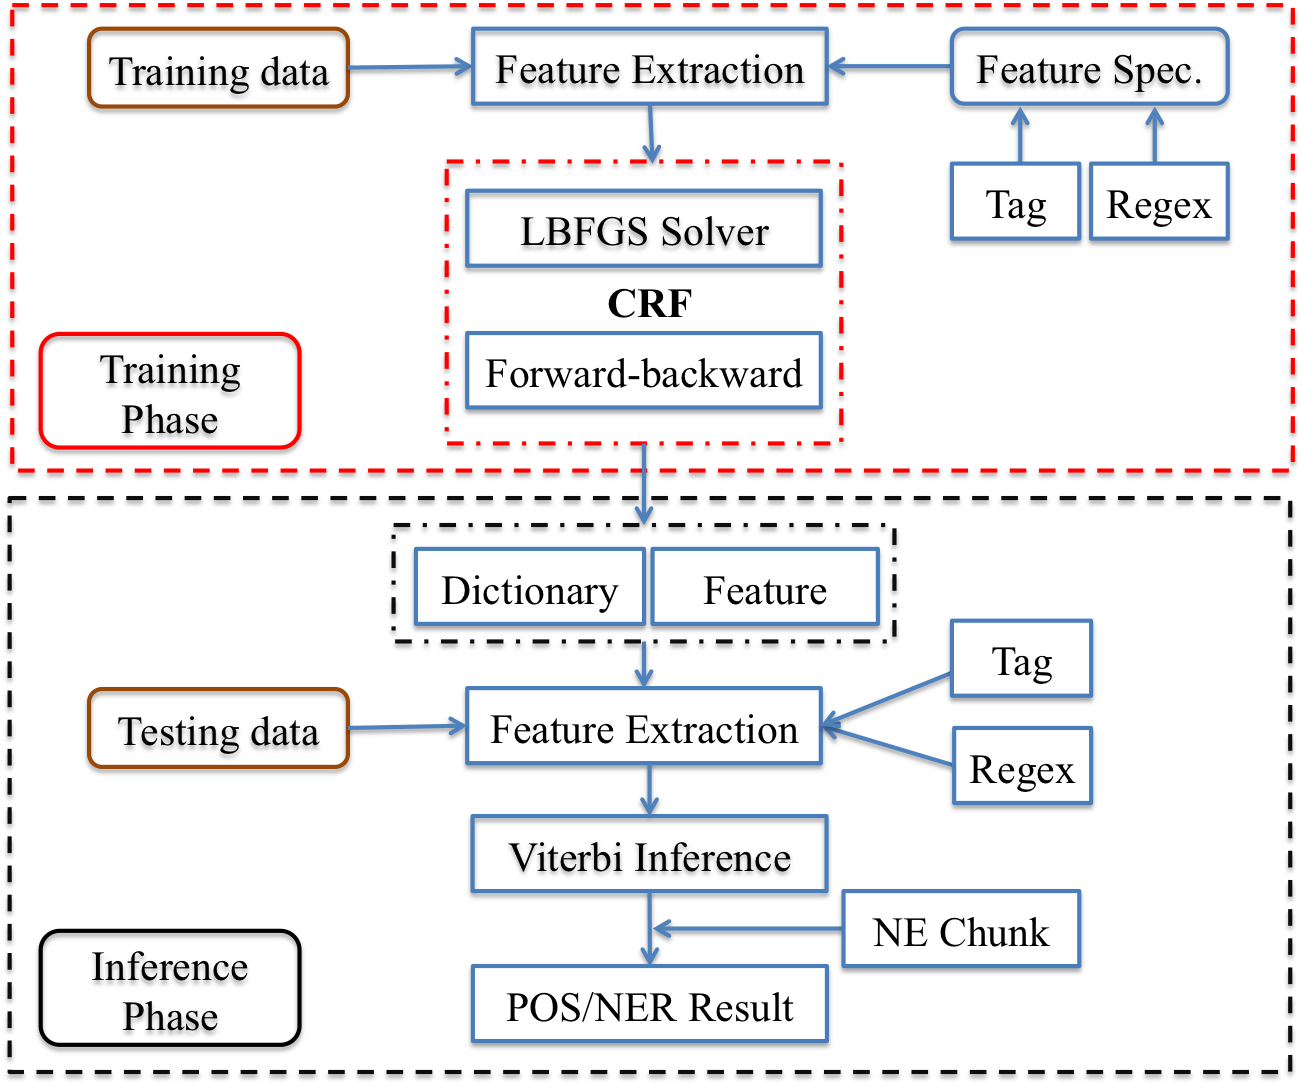
\includegraphics[height=15em]{system.png}
\caption{The MADText overall system architecture.}
\label{fig:systemarch}
\end{figure}

In Figure \ref{fig:systemarch} we show the system architecture for MADText~\footnote{Information on the MABLib library is available at http://madlib.net}. 
The top box contains the shows  the pipeline of the training phase. 
The second box shows the operational pipeline for the inference phase.
In the following sections, we describe each portion of the pipeline.

\subsection{In-database Implementation}
We use declarative SQL statements to extract all features from text.
%Any features in the state of art packages can be extracted using one single SQL clause.
%All of the common features described in literature can be extrated with one  SQL statement.
The extracted features are stored in a relation for either single or two-state features.
%M and R. M table stores the features involves two states. R table store all the single state features.
After the feature extraction, we use user-defined aggregates to calculate the gradient and log-likelihood in parallel using the user defined aggregates.
%We also implement the LBFGS in database. 


\subsection{Feature Extraction Using SQLs}
Text feature extraction is a step in most statistical text analysis methods.
We are able to implement all of the seven types of features used in POS and NER using exactly seven 
SQL statements. These features include: 
\begin{description}[noitemsep]
\item[Dictionary:] does this token exist in a dictionary? 
\item[Regex:] does this token match a regular expression? 
\item[Edge:] is the label of a token correlated with the label of a previous token? 
\item[Word:] does this token appear in the training data?
\item[Unknown:] does this token appeared in the training data below certain threshold? 
\item[Start/End:] is this token first/last in the token sequence?
%\item[End feature:] is this token the last in the token sequence?
\end{description}

There are many advantages for extracting features using SQLs.  
%Compared with procedure language, SQL is much more easier to understand. 
The SQL statements hide a lot of the complexity  present  in the actual operation.
It turns out that each type of feature can be extracted out using exactly one SQL statement, 
making the feature extraction code extremely succinct.  
Secondly, SQLs statements are naively parallel due to the set semantics supported by relational DBMS's.
For example, we compute features for each distinct token and avoid re-computing the features for repeated tokens.  

In Figure~\ref{fig:edgefeatures} and Figure~\ref{fig:regexfeatures} we show how to extract edge
and regex features, respectively.
Figure~\ref{fig:edgefeatures} extracts adjacent labels from sentences and stores them in an array.
Figure~\ref{fig:regexfeatures} shows a query that selects all the sentences that satisfies any 
of the regular expressions present in the table `regextable'.


\begin{figure}
\centering
\begin{lstlisting}[language=SQL,breaklines=true]
SELECT doc2.pos, doc2.doc_id, 'E.', 
       ARRAY[doc1.label, doc2.label]
FROM   segmenttbl doc1, segmenttbl doc2
WHERE  doc1.doc_id = doc2.doc_id AND 
       doc1.pos + 1 = doc2.pos
\end{lstlisting}
\caption{Query for extracting edge features}
\label{fig:edgefeatures}
\end{figure}

\begin{figure}
\centering
\begin{lstlisting}[language=SQL, breaklines=true]
SELECT start_pos, doc_id, 'R_' || r.name, 
       ARRAY[-1, label]
FROM  regextbl r, segmenttbl s
WHERE s.seg_text ~ r.pattern
\end{lstlisting}
\caption{Query for extracting regex features}
\label{fig:regexfeatures}
\end{figure}



\subsection{Parallel Linear-chain CRF Training}
\begin{algorithm} 
\caption{CRF training$(z_{1:M})$} \label{alg:CRF training}
\alginput{$z_{1:M}$, \Comment{Document set}\\
$\mathit{Convergence}()$, \\
%start strategy $\mathit{Start}()$,\\
$\mathit{Initialization}()$,\\
$\mathit{Transition}()$,\\
$\mathit{Finalization}()$}
\algoutput{Coefficients $w \in R^N$}
\algprecond{iteration = 0}
\begin{algorithmic}[1]
%\State $w_{new} \gets \mathit{Start}(z_{1:M})$
\State $\mathit{Initialization}($state$)$ \label{algo:line:traininit}
\Repeat
				\State state $\gets \mathit{LoadState}$() \label{algo:line:trainload}
				%\State state $\gets$ state$_{new}$
        %\State $w_{old} \gets w_{new}$
        %\State state $\gets \mathit{Initialization}(w_{new})$
\ForAll{$m \in 1..M$} \label{algo:line:trainmap} 
\State state $\gets \mathit{Transition}($state$, z_m)$
                %\Comment{Computing gradient and log-likelihood.}
\EndFor
\State state $ \gets Finalization($state$)$ \label{algo:line:trainreduce} %\Comment{Invoke L-BFGS convex solver}
\State $\mathit{WriteState(state)}$ \label{algo:line:trainsave}
\Until{$Convergence($state$, iteration)$}
    \State \Return state$.{w}$ 
\end{algorithmic}
\label{algo:crftraining}
\end{algorithm}

\paragraph{Programming Model.}
In Algorithm~\ref{algo:crftraining} we show the parallel CRF training strategy.
The algorithm is expressed as an user-defined aggregate.
User-defined aggregates are composed of three parts: a transition function (Algorithms~\ref{algo:crftransition}), 
a merge function\footnote{The merge function takes two states and sums their gradient and log-likelihood.},
and a finalization function (Algorithm~\ref{algo:crffinal}).
Following we describe these functions.
%, in the fashion of the selected programming model supported by MADLib (mainly user-defined aggregate).


In line~\ref{algo:line:traininit} of Algorithm~\ref{algo:crftraining} the $\mathit{Initialization}$ function creates a `state' object in the database.
This object contains a coefficient ($w$), gradient ($\nabla$) and log-likelihood ($\mathcal{L}$) variables.
This state is loaded (line~\ref{algo:line:trainload}) and saved (line~\ref{algo:line:trainsave}) between iterations.
We compute the gradient and log-likelihood of each segment in parallel (line~\ref{algo:line:trainmap})  much like a Map function.
Then line~\ref{algo:line:trainreduce} computes the new coefficients much like a reduce function.


%\paragraph{Parallelism.}
%The outer loop is sequential over multiple iterations.
%The iteration $n+1$ takes the output of iteration $n$ as input, so on so forth until the stop criterion is satisfied.
%The inner loop which calculates the gradient and log-likelihood for each document is data-parallel.
%Simple model averaging are used to merge two states.
%%A merge function is not explicitly added to the pseudocode for simplicity.
%The finalization function invokes the L-BFGS convex solver to get a new solution. 
%%L-BFGS is sequential, but very fast.
%%Experiments show that the speed-up ration approaches the number of segments configured in the Greenplum database.

%\paragraph{Convergence criterion.}
%The following convergence criterions are supported.
%\begin{enumerate}
%    \item The norm of gradient divided by the norm of coefficient drops below a given threshold.
%    \item The maximum number of iterations is reached.
%\end{enumerate}

%\paragraph{Start strategy.}
%In most cases, zeros are used unless otherwise specified.

\paragraph{Transition strategies.}
Algorithm~\ref{algo:crftransition} contains the logic of computing the gradient and log-likelihood for each tuple using the forward-backward
algorithm.
This algorithm is invoked in parallel over many segments and the result of these functions are combined using the merge function.
%The algorithms will be discussed in the following sections.

\begin{algorithm}
\caption{transition-lbfgs$(\mathit{state}, z_m)$} \label{alg:transition-lbfgs}
\alginput{state, \Comment{Transition state}\\
$z_m$, \Comment{A Document}\\
$\mathit{Gradient}()$  }
\algoutput{state  }
\begin{algorithmic}[1]
    \State $\{$state.$\nabla$, state$.\mathcal{L}\} \gets \mathit{Gradient}($state$, z_m)$
        %\Comment{using forward-backward algorithm to calculate gradient and loglikelihood}
    \State state$.num\_rows \gets $state$.num\_rows + 1$
    \State \Return state
\end{algorithmic}
\label{algo:crftransition}
\end{algorithm}


%\paragraph{Merge strategies.}
%The merge function takes two states and sums their gradient and log-likelihood.
%The merge function sums the gradient and log-likelihood over all training documents.


%\begin{algorithm}
%\caption{merge-lbfgs$(\mathit{state_1}, \mathit{state_2})$} \label{alg:merge-lbfgs}
%\alginput{Transition state $\mathit{state_1}$,\\
%Transition state $\mathit{state_2}$}
%\algoutput{Transition state $\mathit{state_{new}}$}
%\begin{algorithmic}[1]
%    \State $\mathit{state_{new}}.g \gets \mathit{state_1}.g + \mathit{state_2}.g$
%    \State $\mathit{state_{new}}.loglikelihood \gets \mathit{state_1}.loglikelihood + \mathit{state_2}.loglikelihood$
%    \State \Return $\mathit{state_{new}}$
%\end{algorithmic}
%\end{algorithm}


\paragraph{Finalization strategy.}
The finalization function invokes the L-BFGS convex solver to get a new coefficient vector.\\
\begin{algorithm}
\caption{finalization-lbfgs(state)} \label{alg:CRF training}
\alginput{state,\\
 $\mathit{LBFGS}$() \Comment{Convex optimization solver}}
\algoutput{state}
\begin{algorithmic}[1]
        \State $\{$state.$\nabla$, state.$\mathcal{L}\} \gets $penalty(state.$\nabla$, state.$\mathcal{L}$) %\Comment{To avoid overfitting, add penalization}
        \State instance $\gets \mathit{LBFGS}$.init(state) %\Comment{initialize the L-BFGS instance with previous state}
        \State instance.lbfgs() \Comment{invoke the L-BFGS solver}
        \State \Return instance.state
\end{algorithmic}
\label{algo:crffinal}
\end{algorithm}
%Feeding with current solution, gradient, log-likelihood, etc., the L-BFGS will ouput a new solution.
%To avoid overfitting, a penalization function is needed. We choose to penalize the log-likelihood with a spherical Gaussian weight prior.
%Also, L-BFGS is to maximum objective, so we need to negate the gradient vector and log-likelihood to fit our needs in order minimize the log-likehood.
%\paragraph{LBFGS Convex Optimization}
%The limited-memory BFGS(L-BFGS) is the limited memory variation of the Broyden-Fletcher-Goldfarb-Shanno(BFGS) algorithm which
%is the state of art of large scale non constraint convex optimization method.

Limited-memory BFGS (L-BFGS), a variation of the Broyden-Fletcher-Goldfarb-Shanno (BFGS)
algorithm is a leading method for large scale non-constraint convex optimization method.
We translate an in-memory Java implementation~\cite{morales2000automatic} to a C++ in-database implementation.
%In the in-memory implementation, static variables are defined to pass information to the next iteration.
%However we need to save these variables using a database state object instead of static variables
% for a in-database implementation.
%Eigen vector and Eigen matrix are used instead of the one dimensional and two-dimensional arrays.
%In the Java in-memory implementation, it defines many static variables defined and shared between iterations.
%However, in the MADLib implementation, we define these variables in the state object.
Before each iteration of L-BFGS optimization, we need to initialize the L-BFGS with the current state object. 
At the end of each iteration, we need to dump the updated variables to the database state for next iteration.
 Eigen vectors and Eigen matrices are used instead of the one dimensional and two-dimensional arrays to boost
performance.

%\begin{lstlisting}[language=SQL,gobble=4]
%    select crf_train_data('/path/to/trainingdata')
%\end{lstlisting}

%\begin{lstlisting}[language=SQL,gobble=4]
%    select crf_train_fgen('train_data', 
%    'regex','dic','featuretbl','feature_dic')
%\end{lstlisting}

%\begin{lstlisting}[language=SQL,gobble=4]
%    select lincrf('featuretbl','sparse_r',
%    'dense_m','sparse_m','f_size',45, 
%    'feature_dic','feature',20)
%\end{lstlisting}

\subsection{Parallel Linear-chain CRF Inference}
 The Viterbi algorithm is to find the top-k most likely labellings of a document 
for CRF models. 
We chose to implement a SQL clause to drive the Viterbi inference. 
The Viterbi inference is implemented sequentially and each function call 
will finish labeling of one document.
However, in Greenplum, Viterbi can be run in parallel over different subsets 
of the document on a multi-core machine. So, the CRF inference is naively parallel. 
%\begin{lstlisting}[language=SQL,gobble=4]
%    SELECT doc_id, vcrf_top1(m.score,r.score)
%    FROM   mfactors as m ,rfactors as r
%\end{lstlisting}

%\paragraph{Inference}
%\begin{lstlisting}[language=SQL,gobble=4]
%    select crf_test_data('/path/to/testingdata')
%\end{lstlisting}

%\begin{lstlisting}[language=SQL,gobble=4]
%    select crf_test_fgen('test_data','dic',
%    'label','regex','feature','mtbl','rtbl')
%\end{lstlisting}

%\begin{lstlisting}[language=SQL,gobble=4]
%    select vcrf_label('test_data', 
%    'mtbl','rtbl','label','extraction')
%\end{lstlisting}

%\cite{DBLP:conf/icml/LaffertyMP01}
%\cite{DBLP:journals/scholarpedia/Viterbi09}
%\cite{DBLP:journals/siamjo/MoralesN00}
%\cite{DBLP:journals/coling/DeRose88}
%\cite{DBLP:conf/naacl/ShaP03}
%\cite{DBLP:journals/coling/MarcusSM94}


%\begin{thebibliography}{}
%$\[
%V(i,y) =
%\begin{cases}
%\max_{y^\prime}(V(i-1,y^\prime)) + \textstyle \sum_{k=1}^K \lambda_kf_k(y,y^\prime,x_i), & \text{if } i\ge0 \\
%0, & \text{if } i=-1.
%\end{cases}
%\]$

%\subsection{Entity Detection}

\section{Experiments and Results}
In order to evaluate the performance and scalability of the linear-chain CRF learning and inference on Greenplum,
we conduct experiments on various data sizes over on a 32-core machine with 2T hard drive and 64GB memory.
We use CoNLL2000 dataset containing 8936 tagged sentences for learning. 
This dataset is labeled with 45 POS tags.
%as the tag set. We split the dataset into 6 parts containing 1k, 2k, 4k, 6k, 8k, 9k sentences.
To evaluate the inference performance, we extracted 1.2 million sentences from the New York Times dataset. 
%news and truncated the inference datasets into 5 dataset contains 100k, 200k, 400k, 600k, 800k, 1000k sentences.
In Figure ~\ref{fig:crftrain} and Figure ~\ref{fig:crftest} we show the algorithm is sublinear and improves with an increase in the number of segments.
Our POS implementation achieves $.9715$ accuracy, this is consistent with the state of the art \cite{Manning:2011:PT9:1964799.1964816}.

\begin{figure}
\centering
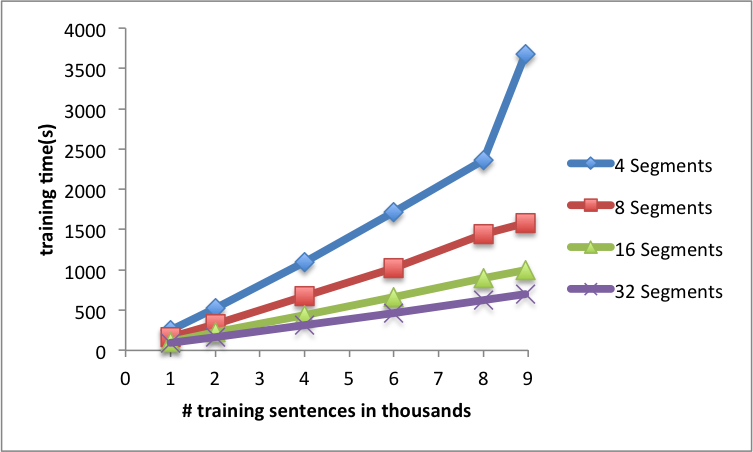
\includegraphics[height=11em]{training}
\caption{Linear-chain CRF training scalability}
\label{fig:crftrain}
\end{figure}

\begin{figure}
\centering
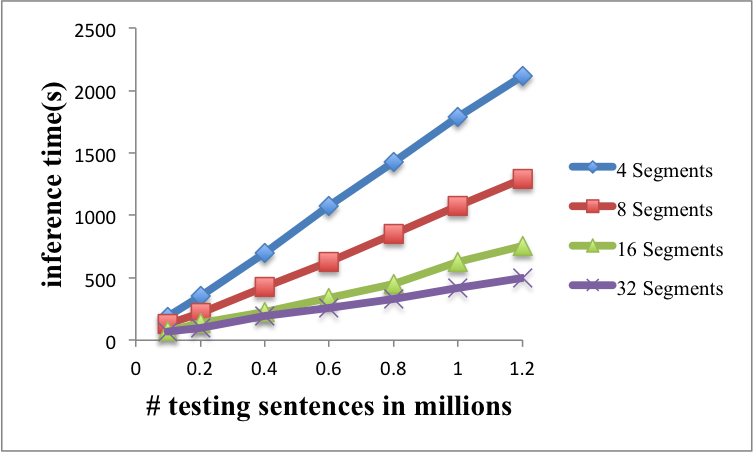
\includegraphics[height=11em]{testing}
\caption{Linear-chain CRF inference scalability}
\label{fig:crftest}
\end{figure}

%\section{User Case: Tweet Analysis}
%\label{sec:blind}

\section{Conclusion and future directions}
We show an approach for using the database as not just the location for
data storage but also as the location for statistical natural language 
computation.
We demonstrate this with the implementation of CRF inference and training 
for part of speech tagging.
We show that these algorithms scale extremely well with the number of cores
in a system.
The RDBMs and SQL interface enable functionalities desired by many 
applications such as real-time training and real-time inference, over
structured and unstructured data.
In the future we plan to support other sophisticated text analytic functionalities,
e.g., parallel Markov Chain Monte Carlo sampling 
for entity resolution in RDBMS.

% TODO We plan on implementing...



\section*{Acknowledgments}
X is funded by a NSF GRF under Grant No. X. %%DGE-0802270.
This work was supported by a gift from a DB company. %EMC Greenplum.

\bibliographystyle{naaclhlt2013}
%\bibliographystyle{plain}
\bibliography{citation}

\end{document}
